\subsection[Diagram klas]{Diagram klas}
\begin{figure}[H]
    \centering
    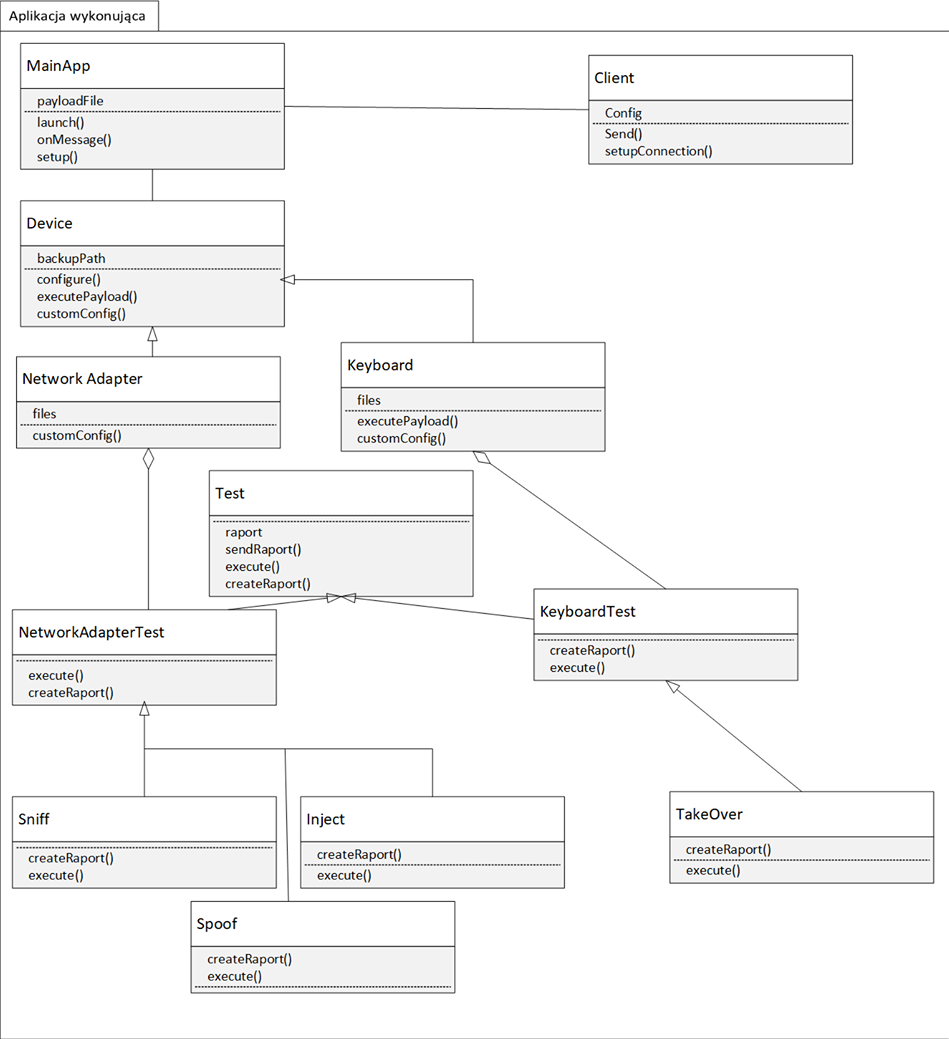
\includegraphics[width=\textwidth]{klaswyk}
    \caption{Diagram klas dot. aplikacji wykonującej}
    \label{fig:klaswyk}
\end{figure}

\begin{figure}[H]
    \centering
    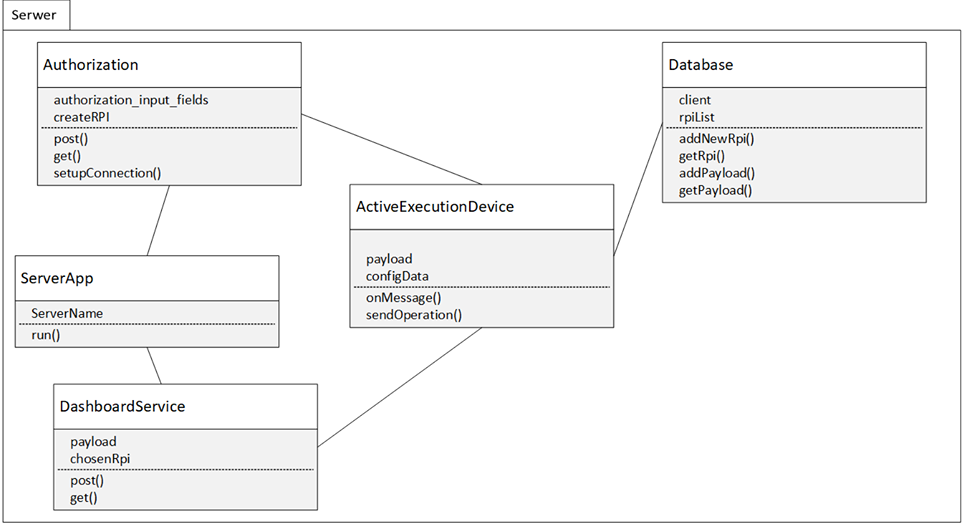
\includegraphics[width=\textwidth]{klasserw}
    \caption{Diagram klas dot. aplikacji serwerowej}
    \label{fig:klasserw}
\end{figure}

\begin{figure}[H]
    \centering
    \includegraphics[width=\textwidth]{klasGUI}
    \caption{Diagram klas dot. interfejsu użytkownika}
    \label{fig:klasGUI}
\end{figure}